\chapter{Propagation of electromagnetic wave inside a parallel waveguide (1)}
Up till now, we have discussed wave propagation in an unbound or semi-bound medium. We have investigated specifically the reflection and refraction of an electromagnetic wave in a dielectric boundary. We saw the reflection of electromagnetic waves from the conducting boundary. Now, we look at the important topic of electromagnetic waves called waveguides. 

\section{Waveguide}\index{Waveguide}
A waveguide is a structure which can guide electromagnetic energy along it. The coaxial cable which we saw in the transmission line is a waveguide structure because it can guide electromagnetic energy from one point to another. The parallel wire transmission line is also a waveguide structure, however, when we go to high frequencies, these waveguides have an excessive loss. This is the reason we get waveguides that are like hollow pipes which are more effective for transmitting electromagnetic energy of higher frequencies. So when we go to frequencies like GHz or tens of GHz, that time the coaxial cable or the parallel wire transmission line, though they have waveguiding characteristics, become lossier and then we stand getting waveguides that look more like hollow pipes with rectangular cross sections or circular cross sections. They can transmit energy from one point to the other more efficiently.

So in communication, waveguides play very important roles. In communication engineering, we are always in search of good waveguide structures that can transfer energy from one point to another at high frequencies. Ideally, a waveguide should have as minimum loss as possible while transmitting the energy from one point to another. The structure should have certain characteristics like:
\begin{enumerate}[(i)]
\item They should be small in size and compact
\item They should be mouldable into desired size and shape so that we can transport the energy easily from one point to another.
\end{enumerate}

When we have a structure like this. we always start with the basis which is Maxwell's equations for the boundary conditions, then we get a solution for a particular problem. However, without going through that routine approach, what we will try to do first is to understand if we still confine ourselves to the uniform plane wave boundaries, can we get a structure like a waveguide structure? That is what we shall do here. With the understanding that we have developed from the reflection of a plane wave from a conducting boundary. We will try to develop an understanding of a waveguide called the \textbf{Parallel Plane Waveguide}. As the name suggests, this waveguide essentially consists of two parallel planes which are of finite distance apart and electromagnetic energy is trapped between these two plane waves. So the energy essentially propagates along this structure trapped between two planes.

\section{Parallel Plane Waveguide}\index{Parallel Plane Waveguide}
In the previous chapter, we took a conducting boundary on which wave was an incident at an angle $\theta$ as shown in figure~\ref{fig:lec35fig1}. The reflected wave made an angle $\theta$ with the normal. By satisfying the boundary condition, we get the reflection coefficient for the electric field. This was $-1$ meaning the conducting boundary was behaving like the equivalent of a short circuit in the transmission line.
\begin{figure}[h]
\centering
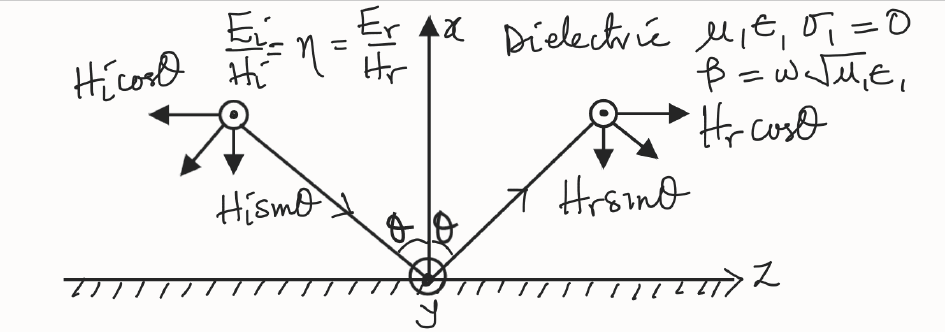
\includegraphics[width=1\linewidth]{./graphics/lec35fig1}
\caption{Incident and reflected electromagnetic wave on a conducting boundary}
\label{fig:lec35fig1}
\end{figure}
The field we had in the dielectric media was a superposition of incident and reflected fields. We obtained an electric field in the medium to be $\bar{E} = \jmath 2E_isin(\beta xcos\theta)e^{-\jmath\beta zsin\theta}$ and $H$ was made up of standing and travelling waves. Here the amplitude of the electric field varies as a sinusoidal pattern in the x-direction perpendicular to the boundary and along the boundary in the z-direction. This is the phenomenon we are going to make use of to get a guiding structure in which electromagnetic energy is not trapped it is travelling in the semi-infinite dielectric medium. If we trap the energy from the two sides we have a parallel plane waveguide. We said the electric field is tangential to the interface at $x=0$, and the tangential component of the electric field should be continuous. We saw that at $x=\frac{m\lambda}{2cos\theta}$, then the electric field at these points becomes zero. Since the electric field had the condition of pointing out or into the paper, i.e. the $\hat{y}$ direction, a conducting sheet placed at $x=\frac{m\lambda}{2cos\theta}$ tangential to this electric field will not affect the boundary conditions. So not only is the tangential component of the electric field 0 at $x=0$ but at some other distance above the interface, the tangential component of the electric field equals zero at $x=\frac{m\lambda}{2cos\theta}$. Hence, the fields which we have got remain unchanged when a conducting sheer is inserted at $x=\frac{m\lambda}{2cos\theta}$. So far $m=0, 1, 2, 3$ we get different values of x at which these boundaries can be inserted without affecting electric or magnetic field distribution. From the graph of variation of $E_y$, $H_x$, and $H_z$ shown in figure~\ref{fig:lec35fig2} with x, we see that at points 1, 2, 3, the field distribution is not affected.
\begin{figure}[h]
\centering
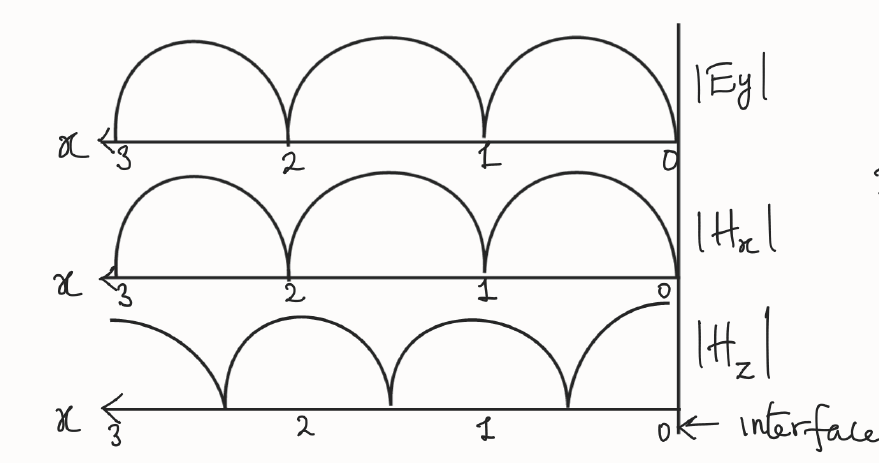
\includegraphics[width=1\linewidth]{./graphics/lec35fig2}
\caption{Variations of components of electric and magnetic fields}
\label{fig:lec35fig2}
\end{figure}

This means that by inserting a conducting sheet at position 1 above the interface, the wave is now trapped between two boundaries. Hence the wave is captured in a form of a closed structure. It is no more a semi-infinite medium. It becomes a bounded medium in the x direction. We can put the conducting plane at 2 or 3 and so on. Here electromagnetic energy is trapped between two parallel planes with a separation between phases given by $x=\frac{m\lambda}{2cos\theta}$. So the new structure is shown in figure|\ref{fig:lec35fig3}. The reflected electric field has the same magnitude as the incident field but goes into the paper contrary to the symbol used for $H$. So we have three components describing the $E$ and $H$ fields. The $E$ field is y oriented, the $H$ has x and z components. The magnetic field is in the xz planes. The electric field (perpendicularly polarized) is oriented tangentially to the plane of incidence. The distance $\frac{\lambda}{2cos\theta}$. So the distance $d=\frac{\lambda}{2cos\theta}$ above the interface, we have the tangential component of the electric field going to zero. At twice this distance $2\left(\frac{\lambda}{2cos\theta}\right)$ from the interface the tangential component of the electric field is zero again. So a place conducting sheet can be placed at any of these distances above the interface plane, without changing the field distribution. When the plane was not at $\frac{\lambda}{2cos\theta}$, fields were distributed at every point above $x>0$. But if a plane conducting sheet is placed at $x=\frac{\lambda}{2cos\theta}$. So we have the propagation of the electromagnetic wave only in the bounded region. So we then have the field surviving in the structure as multiple reflections of the uniform plane wave. They will be bouncing back and forth between the two conducting interfaces or planes. Within these two boundaries with multiple reflections, the wave will travel along the structure or planes.
\begin{figure}[h]
\centering
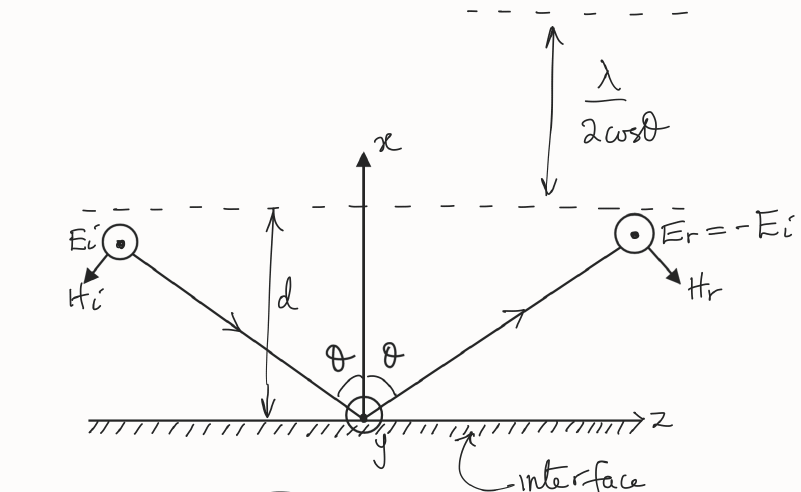
\includegraphics[width=1\linewidth]{./graphics/lec35fig3}
\caption{Incident and reflected electromagnetic wave on a conducting boundary showing the distances when the electric field goes to zero}
\label{fig:lec35fig3}
\end{figure}

Let us invert the problem, i.e. knowing the angle $\theta$, what will be the separation of these planes so that the electric field will not be affected? This is what we have just done. Similarly, given a separation of these two conducting planes as $d$, what angle should the electromagnetic wave be launched such that it can propagate along z or its propagation will be sustained? 
\begin{align*}
d = \frac{m\lambda}{2cos\theta}\\
cos\theta = \frac{m\lambda}{2d}
\end{align*}
$m$ is a discrete number $1, 2, 3, \ldots$. This means that for a given value of d, i.e. a given separation between the two conducting planes, the angel $\theta$ is not continuous, i.e. launching at arbitrary angles which will not sustain the propagation. Only if it is launched at certain angles which are discrete, then and only then can you have a sustained propagation of electromagnetic wave along the structure.

This seems a bit detached from our original understanding of wave propagation in a structure. When we had unbounded media, there was no restriction on the angle, we could launch in any direction. Then in a semi-finite medium (dielectric of the conductor), we could have any angle of incidence and we had semi-field distribution.

\section{Modal Propagation}\index{Modal Propagation}
Now in this case, if we make the structure bound, then an electromagnetic wave cannot be launched at an arbitrary angle of incidence. If we do that, the structure will reject that wave, it will not propagate it. If the wave is launched at the angle which satisfies $cos\theta = \frac{m\lambda}{2d}$ which are discrete angles, then and only then will you have a sustained propagation of what is called a \textbf{Modal Propagation}. So the waves which are launched at discrete angles, superposition of incident and reflected waves will create certain electric and magnetic field patterns within the bound structure. We have a unique pattern created for electric and magnetic fields for a given value of m. For $m=0$, we have a pattern of $E$ and $H$ different form pattern obtained for $m=1$ and so on. $m=1$ gives another pattern of $E$ and $H$ different from that of $m=2$. So we have the discrete electric and magnetic field pattern which can survive inside this bounded structure. This is called \textbf{Modal Propagation} of electromagnetic waves.

So we have migrated now from the continuous domain of $\theta$ to the discrete domain and this is a significant departure we have just encountered in wave propagation. At this point, we can observe a few things, for $\theta$, the $cos\theta$ has to be between 0 and 1, for a given value of $d$, we have a limited number of metres.

When $m$ makes $\frac{m\lambda}{2d}$ greater than 1, that does not represent a physical angle $\theta$. Hence not only that the wave can be launched inside this structure only at discrete angles, we see again that these discrete angles are finite in number. This means that for a given space between the boundaries, only finite numbers of uniform plane waves can be launched given as the number of discrete angles until $\frac{m\lambda}{2d} > 1$.  So this modal propagation is the core of all wave guiding structures whether in parallel, rectangular waveguides, fibre optics etc. Whenever we have a bound medium, the electromagnetic energy is going to travel in definite patterns. That is called a \textbf{Modal Pattern}\index{Modal Patterns} and that propagation is a very important aspect of electromagnetic propagation in a bound structure which is called a waveguide. Once we understand this, finding out the electric and magnetic fields becomes straightforward. So we make some conclusions from all these;
\begin{enumerate}[(i)]
\item Wave survives at discrete angles in a parallel plane waveguide
\item These are a finite number of angles at which the wave survives
\end{enumerate}

With two boundaries, there is nothing like an incident or reflected wave, as an incident wave in one plane is a reflected wave from the opposite plane and vice versa. Depending upon the boundary under consideration, the wave can be called a reflected wave or incident wave.

Hence. with two boundaries, there is nothing like an incident wave or reflected wave as seen in figure~\ref{fig:lec35fig3}. There are two sets of waves which are moving. One set moves up to down (from the top plane to the bottom plane) and another set moves down to up ( from the bottom plane to the top plane). The superposition of these two waves creates a field which is distributed inside the bound structure. This is what is called a \textbf{Modal Pattern}. Shown in figure~\ref{fig:lec35fig4} is what we have essentially with the two sets of waves. The superposition of the fields of these two waves creates the pattern called the modal pattern. Essentially, the propagation of the electromagnetic wave in the bounded structure can be visualized as the superposition of two waves travelling in the pattern shown at an angle with respect to the boundary or perpendicular to the boundary.
\begin{figure}[h]
\centering
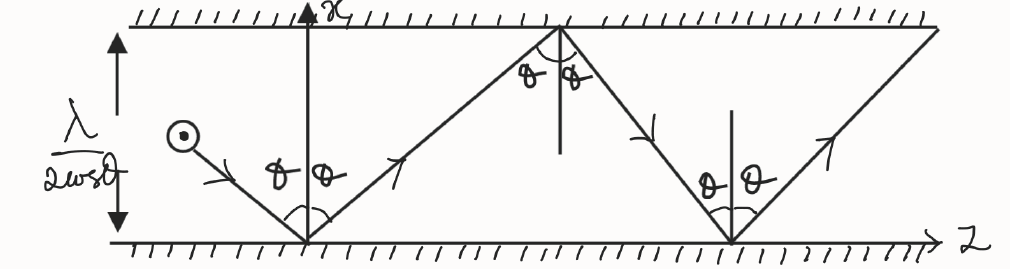
\includegraphics[width=1\linewidth]{./graphics/lec35fig4}
\caption{Wave propagation in a medium of two parallel conducting boundaries}
\label{fig:lec35fig4}
\end{figure}

We observed that in figure~\ref{fig:lec35fig3} with multiple reflections taking place, the net propagation of energy is in the position z direction. The electric field is perpendicular to the plane of incidence i.e. the plane of the paper. So when reflection takes place, the electric field vector maintains the medium. However, the magnetic field direction keeps changing from one point to the other as seen in figure~\ref{fig:lec35fig5}. It shows the direction of $H_i$ and $H_r$ but $E_i$ and $E_r$ remain oriented in the y direction.
\begin{figure}[h]
\centering
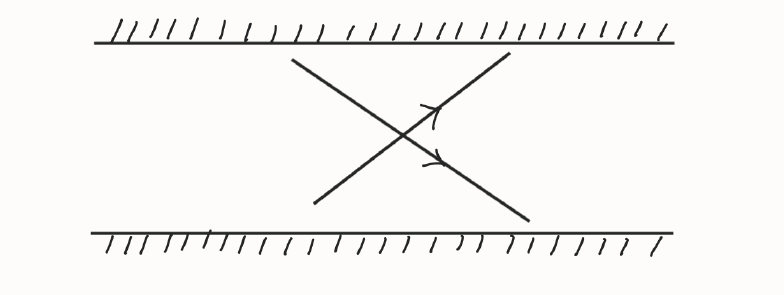
\includegraphics[width=1\linewidth]{./graphics/lec35fig5}
\caption{Wave propagation in a medium of two parallel conducting boundaries showing the superposition of waves}
\label{fig:lec35fig5}
\end{figure}
So $H_r$ and $H_r$ keep changing direction, and the magnetic field inside the plane waveguide has two components, x and z components respectively. Since the net propagation is in the z direction, the magnetic field essentially has components in the direction of net propagation component perpendicular to the direction of net propagation.

Last time
\begin{dmath}
H_x = -\jmath 2\frac{E_i}{\eta}sin\theta sin\left(\frac{m\pi x}{d}\right)e^{-\jmath 2\beta\sqrt{1 - \left(\frac{m\lambda}{2d}\right)^2}}
\end{dmath}
\begin{dmath}
H_z = -\jmath 2\frac{E_i}{\eta}\left(\frac{m\lambda}{2d}\right)cos\left(\frac{m\pi x}{d}\right)e^{-\jmath 2\beta\sqrt{1 - \left(\frac{m\lambda}{2d}\right)^2}}
\end{dmath}
These are the three fields which can survive in a particular waveguide for a perpendicularly polarized electric field (perpendicular to the plane of incidence). Now the phase constant for the mode is
\begin{dmath}
\bar{\beta} = \beta\sqrt{1 - \left(\frac{m\lambda}{2d}\right)^2}
\label{eqn:phaseconst}
\end{dmath}
This is the phase constant as a result of the superposition of two uniform plane waves in the z-direction. $\beta$ is just the phase constant of a single wave moving into the medium.
\begin{dmath}
sin\theta = \sqrt{1-\left(\frac{m\lambda}{2d}\right)^2} 
=\frac{\bar{\beta}}{\beta}
\end{dmath}
The first thing we immediately note from these three expressions is if we put $m=0$, then the electric field goes to zero, $H_x$ goes to zero, and $H_z$ goes to zero. This means that for the fields to survive inside this structure, we must have values of m which is a non-zero integer. Since for $cos\theta = 0$ or $\theta = 90^o$. That means the wave incident on the waveguide cannot survive inside this structure. So if we launched a wave with the electric field shown in figure~\ref{fig:lec35fig6} and with the direction in the y-direction, the wave cannot survive. $E$ is perpendicular to the paper, with $m=0$, the wave cannot survive. 
\begin{figure}[h]
\centering
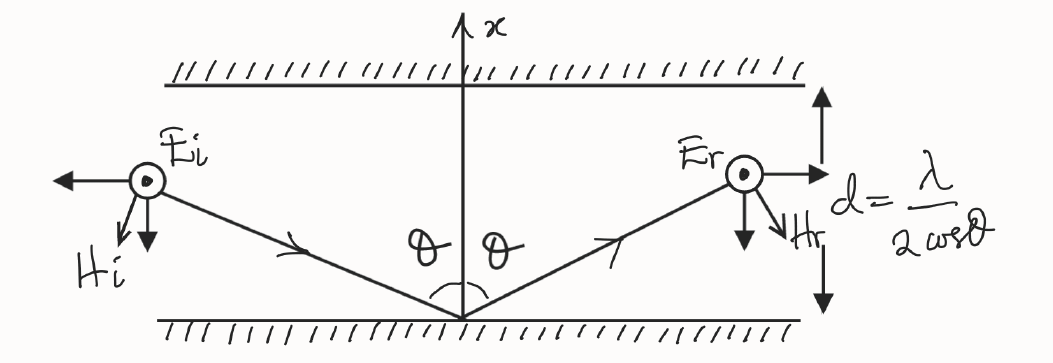
\includegraphics[width=1\linewidth]{./graphics/lec35fig6}
\caption{Wave propagation in a parallel plane waveguide with distance set to $\frac{\lambda}{2cos\theta}$}
\label{fig:lec35fig6}
\end{figure}
Why does this happen? We can see physically from the waveguide structure, m essentially tells us that at $m=1$ and $x=0$ to $d$, we get $\dfrac{1}{2}$ cycle variation of the electric field. So we get the amplitude variation of $E$ shown in the figure~\ref{fig:lec35fig7} for $m=1$, for $m=2$, we have a full cycle variation\footnote{Wondering how it was found, here it is.

At $x=\dfrac{d}{2}$,
\begin{dmath*}
sin\left(\frac{m\pi x}{d}\right) = sin\left(\frac{m\pi \dfrac{d}{2}}{d}\right) = sin\pi = 0
\end{dmath*}}, and for $m=3$, we have $1\dfrac{1}{2}$ cycle variations. 
\begin{figure}[h]
\centering
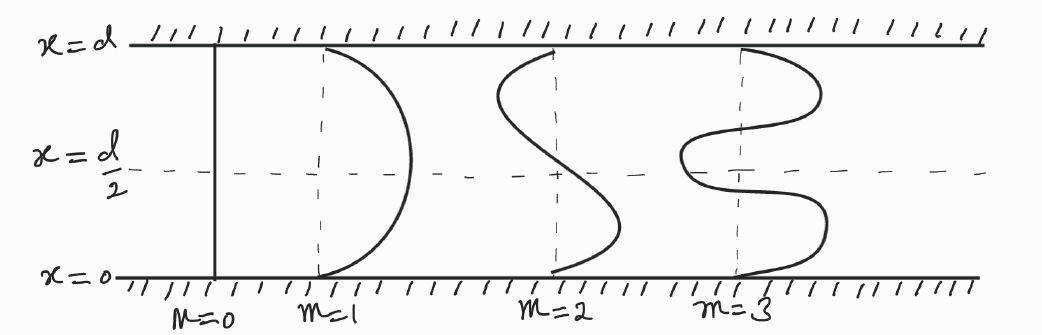
\includegraphics[width=1\linewidth]{./graphics/lec35fig7}
\caption{Electric Field variation with different values of $m$}
\label{fig:lec35fig7}
\end{figure}

So m tells us how many half cycles variations of the electric field amplitude or magnetic field amplitude in the direction transverse to the direction of net wave propagation. So if $m=0$, there is no variation which means a constant field from $x=0$ to $x=d$. $m=1$ means 1 half-cycle variation, $m=2$ means 2 half-cycle variations, $m=3$ means 3 half-cycle variations and so on. For $m=0$ the field is constant in the direction transverse to the direction of propagation. Since the electric field is in the y direction, between two conducting planes, at the conducting boundaries, the electric field must be zero at both of them. For $m=0$ we do not want any variation of the field and it should be zero at $x=0$ and $x=d$.That will only happen if the field is identically zero everywhere. That is what the bold part of the expression, $\bar{E} = \jmath 2E_i\boldsymbol{sin\left(\frac{m\pi x}{d}\right)}e^{-\jmath 2\beta\sqrt{1 - \left(\frac{m\lambda}{2d}\right)^2}}$, tells us. So the lowest value of m which can survive in the structure is $TE_1$ mode. Hence, for a given spacing of conducting planes, we must have a value, m, which is at least 1 and only then will the field exist in the structure, if $m=0$ the field will not exist inside the structure and the wave will not propagate. So depending upon the size or mode, we can have $TE_1$, if the size is sufficient, $TE_2$, $TE_3$ and so on.

On a given structure, we can have multiple modes propagating depending upon how the angles $cos\theta = \frac{m\lambda}{2d}$ can be satisfied. $m=1$ is the lowest mode, so the question is what wave can survive in mode 1? With $cos\theta = 1$, $\dfrac{m\lambda}{2d} = 1$, hence, $\lambda = 2d$ or $d = \dfrac{\lambda}{2}$. This implies that the separation between the planes is $\dfrac{\lambda}{2}$. Thus in $TE_1$ mode the smallest separation is $\dfrac{\lambda}{2}$, if it is less than $\dfrac{\lambda}{2}$, we cannot have an angle as $\dfrac{m\lambda}{2(0.4\lambda \text{ assume})}> 1$, so that $cos\theta > 1$. No physical angle has its cosine greater than 1. So the lowest mode for which the wave can propagate in the structure has $d \geq \dfrac{\lambda}{2}$\footnote{This makes $cos\theta \leq 1$}. So not only that the separation distance $d$ is given, but a wavelength is required for which $d\geq\dfrac{\lambda}{2}$ or inverted $\lambda \leq 2d$. This means the frequency has to be above certain values so that $\lambda \leq 2d$ is satisfied, only then will the wave propagation take place. If $\lambda > 2d$ or frequency is less than certain values, then wave propagation cannot take place inside the structure.

\section{Trough of a mode}\index{Trough of a mode}
 So from here, we get an important concept of what is called the \textbf{Trough} of a mode, that is when $d = \dfrac{\lambda}{2}$ or $\lambda = 2d$ which is the lowest frequency that can propagate on a waveguide whose separation is $d$.
\begin{dmath}
\lambda_{max} = 2d
\label{eqn:cut-offlambda}
\end{dmath}
\begin{dmath*}
\frac{c}{f_{min}} = 2d
\end{dmath*}
\begin{dmath}
f_{min} = \frac{c}{2d}
\label{eqn:cut-offf}
\end{dmath}
Equations \ref{eqn:cut-offlambda} and \ref{eqn:cut-offf} are the maximum wavelength and minimum frequency respectively that defines wave propagation. Below $f_{min}$, the wave doesn't propagate and that is the minimum frequency for $m=1$ mode and it is called the cut-off frequency of that mode. So for a particular mode to propagate the frequency must be above that value and that is called the cut-off frequency for that mode.

The cut-off frequency is the lowest frequency which would propagate inside the structure for a given mode number or given $m$. Either we see that or the mode increases to $TE_2$, the frequency will be doubled and so on. Hence the reason we say the lowest mode is because that is the lowest frequency in the structure which can propagate.

Substituting $d=\dfrac{\lambda}{2}$ and $m=1$ in equation ~\ref{eqn:phaseconst} gives:
\begin{dmath*}
\bar{\beta} = \beta\sqrt{1 - \left(\frac{m\lambda}{2d}\right)^2} =  \beta\sqrt{1 - \left(\frac{\lambda}{2\left(\frac{\lambda}{2}\right)}\right)^2} = 0
\end{dmath*}
This shows that the frequency at $d=\dfrac{\lambda}{2}$ which is the cut-off frequency, the phase constant of the wave goes to zero. Below this frequency $\left(\dfrac{m\lambda}{2d}\right)^2 > 1$, the expression $\sqrt{1 - \left(\frac{m\lambda}{2d}\right)^2}$ in the phase constant is imaginary, so $\bar{\beta}$ becomes imaginary. It is no more a phase constant but becomes an attenuation constant i.e. the wave losses its wave nature in the presence of a field which is dying down exponentially. So below the cut-off frequency, it represents a field which is exponentially decaying and hence no propagation of electromagnetic waves.

What we see from this analysis is that when we have a band structure like a parallel plane waveguide, first there are the discrete angles at which uniform plane waves are bouncing back and forth between two parallel planes giving the field distribution and those field patterns we call modal patterns. We also see that for a given mode number, the frequency has to be above certain values called cut-off frequency for that mode. So depending on the mode you want to excite, you require a certain frequency. So even if the waveguide is capable of supporting the different values of $m$, it would depend on the frequency whether the wave will be accepted or not i.e. if the frequency is greater than the cut-off frequency or not. This is the basic picture of modal propagation within a bounded structure like a waveguide. We will elaborate on this and then following this, we will try to see other modes and then move on to complex structures like the rectangular waveguides.